\documentclass[a4paper,10pt,twoside,openany]{article}
\usepackage{graphicx}
%\usepackage{fancyhdr}
\usepackage{xcolor}
\usepackage{ifpdf}
\usepackage{ifthen}
\usepackage[round]{natbib}
\usepackage{amsmath}







%%set font
\usepackage[T1]{fontenc}
%and allow UTF8 input ( e.g. umlauts and friends)
\usepackage[utf8]{inputenc}
\usepackage{palatino}
\usepackage{mathpazo}
%\usepackage{utopia}
%\usepackage{euler}


%define some colors
\definecolor{gfzblue}{rgb}{0., 0.4, 0.65}
\definecolor{iggblue}{rgb}{0,0.258824,0.568627}
%or gray
\definecolor{graycust}{rgb}{0.45,0.45,0.45}

\definecolor{backgrnd}{rgb}{0.8, 0.8, 0.8}
\definecolor{sunsetorange}{rgb}{1, .3, .11}
\definecolor{mossgreen}{rgb}{0.14,0.5,0.06}

%% Search path for figures
\graphicspath{{figs/}} %% full color figures
%%\graphicspath{{figures_gray/}} %% for grayscale figures

%%


%new commands to insert the title subtitle and author where necessary
\newcommand{\ititle}{Surface Loading effects on the LHC tunnel}
\title{\ititle}
\newcommand{\iauthor}{Roelof Rietbroek}
\author{\iauthor}

%add command to quickly insert colored remarks in the margin
\newcommand{\todo}[1]{\marginline{\color{red} TODO:\\#1}}

%pdf vs non-pdf options
\ifpdf
   \usepackage[pdftex,pdfpagelabels]{hyperref}
   \pdfcompresslevel=9
   \hypersetup{
     pdftitle={\ititle},
     pdfauthor={\iauthor},
     pdfsubject={LHC tunnel deformtions},
     pdfkeywords={Geodesy},
     colorlinks=true,
     urlcolor=iggblue,
     linkcolor=iggblue,
     citecolor=iggblue,
     breaklinks=true,
     plainpages=false
   }

\else
  \usepackage{hyperref} %basic dvi output with fugly  but obvious hyperlinks
     \hypersetup{
     colorlinks=true,
     urlcolor=iggblue,
     linkcolor=iggblue,
     citecolor=iggblue,
     breaklinks=true,
     plainpages=false
     }                           
  
\fi


%includeonly
%\includeonly{preface}
% begin main document
\begin{document}
\maketitle

\section{Introduction}
Some thoughts and a theoretical framework are gathered here to
quantify the circumference changes due to surface loading induced
deformations of the bedrock.

\section{Horizontal deformations due to surface loading}
\section{LHC circumference changes due to horizontal surface
  deformations}
Assumptions:
\begin{itemize}
\item ring is positioned horizontally (it is only approximately horizontal)
  is)
  \item Horizontal deformations in and around the ring can be
    linearized wrt to the center point.
\end{itemize}
\begin{figure}
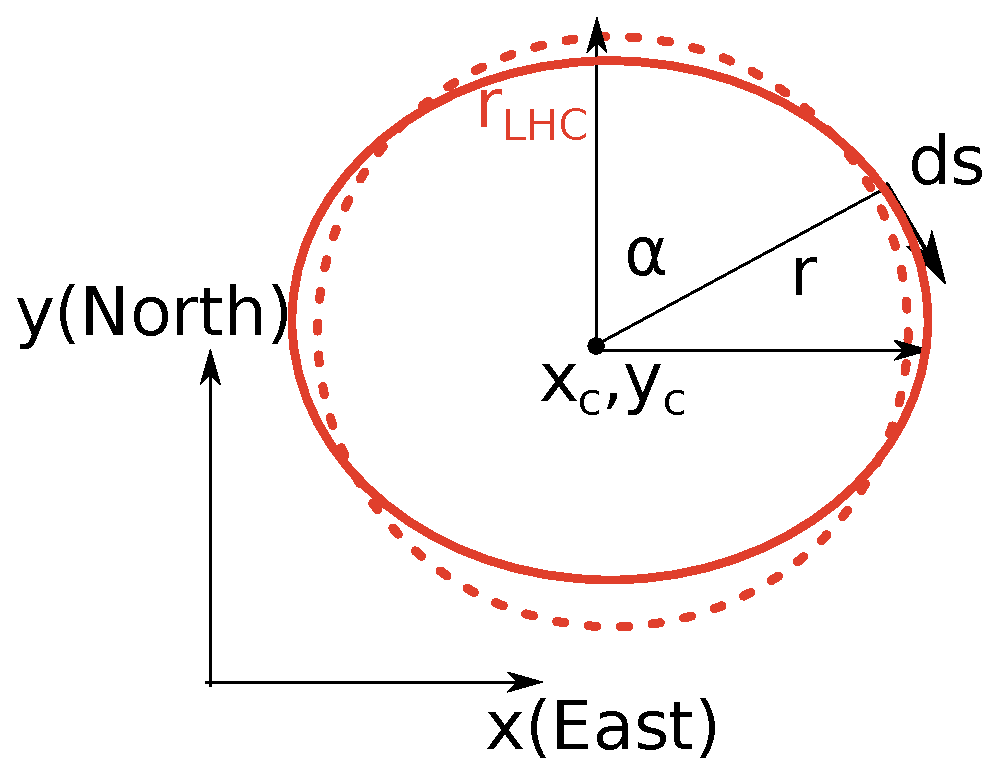
\includegraphics[width=\textwidth]{Ringschematically}
\end{figure}
The circumference of the LHC ring,  $\Delta L$, may be computed by a path
integral over the ring which is deformed from a perfect circle by $\vec{h}(x,y)$:
\begin{equation}
  L =\oint_{deformed ring} ds(x,y) 
\end{equation}
We parameterize the path of deformed ring in terms of angle
$\alpha$. The infinitesimal path length $ds(x,y)$ , can then be
linked to $d\alpha$ by:
\begin{equation}
r\alpha=\vec{e}_{\alpha}\cdot (\vec{e}_{s} ds)
\end{equation}
Where $\vec{e}_{s}$ is the tangential (unit) vector to the deformed ring and
$\vec{e}_{\alpha}$ is a unit vector in the direction of alpha:
\begin{equation}
\vec{e}_{\alpha}=\left[\begin{array}{c}\cos \alpha\\-\sin \alpha\end{array}\right]
\end{equation}

The integral above may thus be rewritten in terms of $\alpha$.
\begin{equation}
  L =\int_{0}^{2\pi} \frac{r}{\vec{e}_{\alpha}\cdot \vec{e}_{s}}d\alpha 
\end{equation}


There are several approximations which we can now apply:
\begin{itemize}
  \item linearize the horizontal deformation field around the center
    of the ring. (Probably OK, since the deformations are expected to
    be of large scale (10s of kms').
    \item evaluate  the horizontal deformations at the original ring
      and not on the deformed ring. This may help in solving the
      integral  in an analytical way.
  \end{itemize}

%%For a circular  ring we may parameterize the ring in terms of a fixed
%% radius, $r_{lhc}$ and an azimuth angle $\alpha$:
%% \begin{equation}
%%   \Delta L =\int_{0}^{2\pi}
%%   \left[\begin{array}{c}h_{x}(x,y)\\h_{y}(x,y)\end{array}\right]
%%   \cdot \left[\begin{array}{c}\cos \alpha\\-\sin \alpha\end{array}\right]d\alpha
%% \label{eq:2}\end{equation}


%% When the  ring is relatively small we may linearize the deformation
%% around the ring's center $(\lambda_{c},\theta_{c})$:
%% \begin{equation}
%% \vec{h}(x,y)=\vec{h}(x_{c},y_{c})+\frac{\partial \vec{h}}{\partial
%%   x}\vert_{c}(x-x_{c})+ \frac{\partial \vec{h}}{\partial y}\vert_{c}(y-y_{c})+ \mathcal{O}(2) 
%% \end{equation}

%% noting that:
%% \[
%% \left[\begin{array}{c}x-x_{c}\\y-y_{c}\end{array}\right]=r_{LHC}\left[\begin{array}{c}\sin \alpha\\\cos \alpha\end{array}\right]
%% \]
%% We can solve the integral \ref{eq:2} in terms of the gradients of the
%% horizontal deformation field:
%% \begin{equation}
%% \Delta L=
%% \end{equation}
\subsection{Hydrology and atmospheric induced LHC circumference changes from GRACE data}
\subsection{LHC circumference changes due to water level changes}



% make Bibliography
%% \bibliography{roelofsrefsauto}
%% \bibliographystyle{abbrvnat}
%\bibliographystyle{plainnat}
%\bibliographystyle{authordate1}
\end{document}

